\chapter{Planteamiento del Problema}

%* Agregar un párrafo introductorio donde se informe al lector que se encontrará en el capítulo.

Las redes de monitoreo de meteorológico y de calidad del aire de alta densidad son una necesidad creciente de las áreas urbanizadas, las cuales necesitan de una infraestructura cada vez más compleja para su monitreo y seguimiento. Estas necesidades crecientes de infraestructura han generado una demanda creciente de recursos humanos, y la falta de homogeneidad entre las estaciones de monitoreo presentan retos a conquistar para proveer servicios cada vez más sofisticados. En este capítulo, se discutirá la importancia de la infraestructura de monitoreo y se explicarán los diferentes métodos de monitoreo que existen actualmente para monitorear las estaciones meteorológicas, así como una propuesta de solución para los problemas que los sistemas tradicionales existentes presentan.

\section{Antecedentes}

El desplegar y mantener una red meteorológica urbana compone bastantes retos: Entre la creciente dificultad de crear sistemas de medición estandarizados que se adapten al siempre cambiante paisaje urbano; como la instalación de los equipos de medición y de guardado de datos en áreas que permitan acceso para mantenimiento y que sean seguros; y la dificultad de encontrar un punto de acceso a internet adecuado para transferir la información generada, el generar una red de monitoreo es una tarea extensa y compleja.

Debido a estos retos, la comunidad de monitoreo climatológico y meteorológico se ha enfocado en la creación de sistemas que sean más eficientes y económicos. Entre estos esfuerzos, se encuentra el amplio uso de RaspberryPi como centro de recolección de datos de estaciones de monitoreo \cite{rpi_weataher_station}, tanto caseras como profesionales, con la ayuda de sistemas abiertos para la recolección de datos como lo es WeeWX. Esto ha hecho factible el \textit{levantar} redes de 50 nodos de monitoreo con sensores económicamente viables para actores con un presupuesto limitado \cite{monitoreo_raspberry_nagios}.

% TODO Levantar, en el parrafito anterior no me agrada por completo, pero lo dejo debido a la falta de una mejor palabra.

% TODO! Agregar sección de monitoreo de Campbell, y como funciona actualmente. Port forwarding en Campbell, porque no están en nuestra red.

%! Las estaciones están en la sierra, hacer diagnóstico remoto.

%! Davis Weatherlink Live. https://www.davisinstruments.com/weatherlinklive/

%! IMPORTANCIA A REDES HETEROGÉNEAS, no tanto a porque davis funciona como funcione, sino por las redes heterogéneas.

Estas redes densas requieren de un monitoreo contínuo para mantener una alta calidad de los datos recabados, y evitar las pérdidas por falta de mantenimiento. Entre los sistemas de monitoreo que pueden ser adaptados para el monitoreo de estaciones meteorológicas y la red que las soporta, se encuentra la plataforma Nagios®, el cual es un sistema de monitoreo contínuo orientado a redes y servidores. Entre la información que recaba Nagios contínuamente para el estado de los servidores, se encuentra el uso de CPU y RAM, así como estado de los discos, puertos, e información variada de servicios de red en los hosts. Debido a que Nagios es un sistema de monitoreo de redes orientado a profesionales de la informática, la interfaz gráfica es poco amigable con los usuarios menos familiarizados con los conceptos técnicos de los sistemas computacionales, como se muestra en la Figura \ref{fig:nagios_dashboard}.

\begin{figure}[!ht]
	\centering
	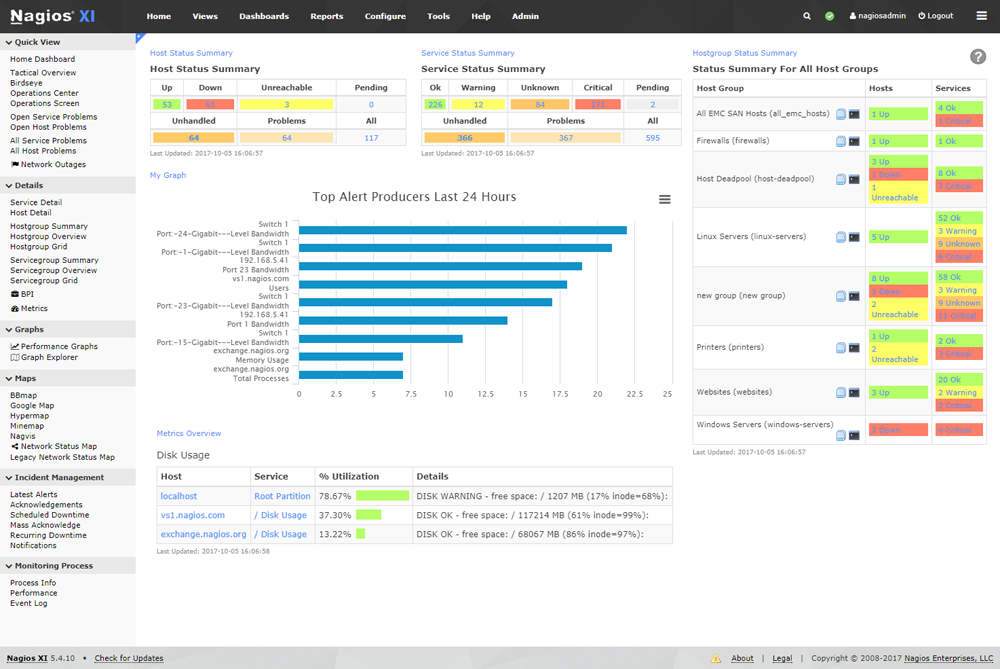
\includegraphics[width=.80\linewidth]{images/Nagios_home_dashboard.png}
	\caption{Tablero principal de Nagios XI.}
	\label{fig:nagios_dashboard}
\end{figure}

Si bien Nagios ofrece la posibilidad de monitorear parámetros adicionales con un sistema establecido de plugins en python y otros lenguajes, además de poseer una fuerte comunidad que crea contínuamente plugins relacionados con el proyecto, hasta el momento la cantidad de plugins relacionados con estaciones meteorológicas existentes es mínima ya que los esfuerzos de la comunidad se centran principalmente en el monitoreo de centros de datos, redes y routers.

Además de los plugins existentes en la comunidad de Nagios, existe la alternativa abierta conocida como \textit{monitoring plugins} \cite{monitoring_plugins}, que es una plataforma compatible con diversos sistemas de monitoreo de redes y servicios, en la cual es posible encontrar una mayor cantidad de scripts de monitoreo relacionados con los sistemas de recolección de datos meteorológicos. La utilización de estos \textit{plugins abiertos} junto con un sistema central como Nagios ya ha sido propuesto anteriormente \cite{monitoreo_raspberry_nagios}.

% Definir plugins abiertos, colocarlo como itálica
% Scripts

Las limitaciones de Nagios vienen a que debido a su implementación orientada a sistemas de alta disponibilidad, la configuración de los parámetros de tolerancia para la resilencia a fallas son generalmente limitados en la variedad de los mismos y los valores fijos que se pueden establecer. Además, debido a las necesidades de seguridad y accesibilidad de las estaciones meteorológicas en el contexto urbano, estas suelen instalarse en sistemas en los que se posee poco control de la red que les provee comunicación, como son las escuelas, hospitales y estaciones de policía, así como otros espacios públicos \cite{muller_sensors_and_the_city}, dificultando aún más la capacidad de monitoreo y disponibilidad de la red y los sistemas que soporta. Esta limitante se hace más presente debido a que los sistemas se vuelven completamente dependientes de una VPN para funcionar y para su control, debido al extenso uso de redes NAT IPv4 que predominan en los sitios de instalación.

Otra de las limitantes del sistema Nagios es que al ser un sistema de monitoreo limita la capacidad de acción de los usuarios ante un caso que lo requiera. Si bien es posible el realizar acciones por medio de scripts creados al momento de la configuración de Nagios, estos requieren una configuración extensa y compleja \cite{nagios_service_restart}. Además, el sistema basado en eventos impide la interacción directa de un usuario para la respuesta de forma directa desde la consola de administración, requiriendo que el usuario tenga un conocimiento del método de conexión así como la información necesaria para realizar una tarea trivial como es el reiniciar un servicio.

% Pero de la misma forma, al ser un equipo de cómputo con funciones específicas, requiere de un alto grado de entendimiento de las funciones que realiza para poder modificarlas, así como un diagnóstico detallado y complicado para poder repararlas en caso de un fallo.

% Debido a la *[disponibilidad e integridad]* de los datos requerida en las estaciones meteorológicas, han buscado crear redes resilentes [...], pero eso no evita que sean completamente resistente a fallos.

%! Las estaciones meteorológicas son redes heterogéneas ¿A que me refería con esto?

Actualmente, el sistema de monitoreo de calidad del aire y climatológico de la Universidad Autónoma de Ciudad Juárez, engloba varios de los retos antes descritos, ya que a pesar de la baja densidad de estaciones meteorológicas, comprende una variedad importante de las mismas. Actualmente, se compone por prototipos conectados por medio de puertos expuestos por NAT monitoreados remotamente \cite{red_climatologica_uacj}, estaciones de diferentes proveedores siendo monitoreadas local y externamente, así como estaciones remotas con routers dentro de la red local de la universidad (véase la Figura \ref{fig:current_network}). Lo que provoca que sea un reto el monitorearla adecuadamente debido a la variedad de sus componentes.

\begin{figure}[!ht]
	\centering
	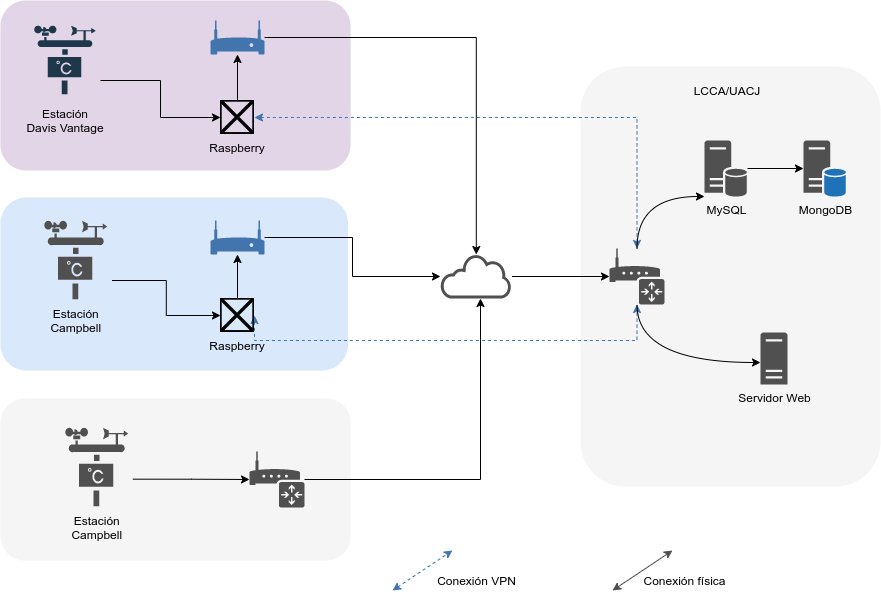
\includegraphics[width=.80\linewidth]{images/diagrams/current_network.png}
	\caption{Diagrama de red de LCCA UACJ.}
	\label{fig:current_network}
\end{figure}

%! Hay estaciones Vantage y Vantage Pro, las Campbell trabajan con el CR100, y hay unas que se conectan al CR100 desde la raspberry pi.

Una parte vital de los sistemas de monitoreo es el registro detallado de incidentes para su posterior análisis o referencia y actualmente, no se cuenta con un registro de causas y soluciones, una base de conocimientos para los fallos de las estaciones meteorológicas existentes, así como tampoco existe un reporte automático de la calidad de los datos meteorológicos derivado de los diagnósticos y estado de salud de las estaciones meteorológicas, lo cual dificulta el uso de la información recabada por las mismas por los usuarios que accedan a la información que es recabada.


\section{Definición del problema}

La falta de una plataforma estandarizada para el monitoreo de estaciones meteorológicas que permita un monitoreo contínuo y control de diversos tipos de estaciones, así como la disponibilidad del acceso a los datos, y un registro de incidentes crea una dificultad creciente para los administradores de redes de monitoreo meteorológico. Con redes cada vez más densas que son cada más accesibles económicamente y menos complejas de crear, se hace notar la necesidad de un sistema estandarizado y compatible con soluciones existentes para el monitoreo de las estaciones.

%* ¿A qué tipo de redes me refiero?

%! Mejores tiempos de respuesta como aporte secundario en la metodología, esto es complicado de medir debido a que falta información.

\section{Objetivo general}

Desarrollar un sistema de monitoreo y control para estaciones meteorológicas que permita un monitoreo contínuo de las mismas por parte de personal no especializado, con el objetivo de proveer un mejor mantenimiento preventivo y correctivo de las estaciones meteorológicas y de calidad del aire.

%* ¿Doble uso de palabra monitoreo? ¿Monitoreo contínuo DEL personal?

%! Mi propósito principal es proveer fácil administración y diagnóstico de forma remota.

\subsection{Objetivos específicos}

\begin{itemize}
   %! \item Hacer un sistema modular y extendible para el monitoreo de las estaciones meteorológicas.

   \item Desarrollar un sistema central para coordinar y recolectar los datos del estado de las estaciones.

   \item Diseñar un API REST para consultar el estado de las estaciones meteorológicas.

   %! Agregar como subobjetivo una base de conocimientos. (como lo justifico?) Demostrar tiempos de respuesta para QAPP.
   %! Herramientas de gestión de calidad
   %! Personas como parte de gestion

   \item Diseñar e implementar una interfaz gráfica para monitorear el estatus de las estaciones.

   \item Integrar las diferentes estaciones meteorológicas existentes al sistema creando los controladores correspondientes.

   \item Integrar un sistema existente de notificaciones/alertas de terceros para fallos críticos de las estaciones.
\end{itemize}

\section{Justificación}

Creando un sistema de monitoreo eficaz para las estaciones meteorológicas se pretende el alcanzar una mayor calidad de los datos obtenidos de las mismas, así como una mejor documentación de los sistemas meteorológicos por consecuencias. Esto pretende dar el tiempo al personal especializado en enfocarse en expandir las redes existentes meteorológicas, mejorando a largo plazo la calidad y la definición de los datos recabados con la misma cantidad de esfuerzo.

Además, haciendo el sistema de monitoreo un proyecto público y compatible con soluciones existentes, se pretende el ayudar a mejorar la calidad y confiabilidad de las redes de monitoreo meteorológico, de calidad del aire y climatológico al rededor del mundo.

%! Impacto en la justificación! Que impacto tiene mi proyecto?
%! Indicar el porqué

%! Series contínuas de datos de calidad
% Cambio climático, sequías. A pesar de que ya hay muchos datos (por ejemplos satelitales), no tenemos bases de datos con series de tiempo de buena calidad de series de los datos. Y esto tiene que ver con la cada vez más limitada capacidad de mantener la red y darle mantenimiento. A veces no hay los recusos para ir físicamente, el tiempo, o la información de los datos.

% Se tarda mucho tiempo en visitar las estaciones, hacer un uso extensivo de las capacidades tecnológicas actuales.

\subsection{Alcances y limitaciones}

%* Presentar alcances y imitaciones en forma de lista

%! Los alcances son los aspectos que voy alograr, limitaciones son los aspectos que no voy a lograr.

Entre los alcances que pretende tener el proyecto, se tienen contemplados los siguientes:

\begin{itemize}

   \item Integrar estaciones meteorológicas existentes, que se encuentren conectadas a la red de comunicaciones del CECATEV ya sea directamente o por medio de una VPN.
   \item Se entregará un sistema instaldo, funcional y listo para monitorear las estaciones seleccionadas, sin necesidad de configuraciones extraordinarias.

\end{itemize}

Si bien se pretende que el proyecto tenga la flexibilidad suficiente para adaptarse a nuevos casos de uso sin necesidad de reescribir grandes partes del mismo, también se consideran las siguientes limitaciones:

\begin{itemize}

\item La integración se limitará a cubrir casos conocidos y recurrentes de estaciones meteorológicas existentes.
\item Sólo se considera integrar una estación meteorológica de cada tipo en cada topología, dejando como proyecto futuro integrar la totalidad de la red de la universidad.
\item El sistema se limitará a cubrir los casos de fallas comunes y conocidos de las estaciones.
\item Sólo se monitorearán los servicios básicos de las estaciones meteorológicas que son vitales para el funcionamiento.

Servicios tales como:

\begin{itemize}
   \item Servicios el cliente de VPN para estaciones que así lo requieran.
   \item Servicio de copias de respaldo (si aplica).
   \item El servicio de monitoreo climático WeeWX.
\end{itemize}

\end{itemize}

% La integración de estaciones meteorológicas se limitará a cubrir casos conocidos y recurrentes de estaciones meteorológicas existentes, como lo son las estaciones Davis Vantage Pro® conectadas a un RaspberryPi como DataLogger, así como las estaciones Campbell® accesadas directamente por su dirección IP y a las que se accesa por medio de una RaspberryPi que funciona como DataLogger. El proyecto estará limitado a conectarse a solamente una de cada uno de los tipos de estaciones meteorológicas existentes.

% Así mismo, la interfaz gráfica, y el diseño y la implementación del API se limitarán a cubrir los casos comunes de fallo de las estaciones anteriormente mencionadas. Respecto a los servicios que el sistema monitoreará, se pretende que sólo se monitoreen los escenciales para el monitoreo y funcionamiento correcto del sistema de recolección de datos existentes, tales como el servicio WeeWX, el proveedor de VPN y el servicio de backups por estación si es que existe. De la misma forma, el proyecto se limitará a adaptarse a la infraestructura de red existente y a integrar estaciones que se encuentren recolectando datos.
